

\chapter[ICA on the Sphere]{Independent Component Analysis on the Sphere}
\label{ch_mrs_ica}


\section{Introduction}
\index{blind source separation}
\index{ICA}


Blind Source Separation (BSS) is a problem that occurs in multi-dimensional data processing. The overall goal is to recover 
unobserved signals, images or \emph{sources} $S$ from mixtures of these sources $X$ observed typically at the output of an 
array of sensors. The simplest mixture model takes the form:
\begin{equation}\label{model0}
X = A S
\end{equation}
where $X$ and $S$ are random vectors of respective sizes $m \times 1$, $n \times 1$ and $A$ is an $m \times n$ matrix. The 
entries of $S$ are assumed to be independent random variables. Multiplying $S$ by $A$ linearly mixes the $n$ sources into 
$m$ observed processes. \\ 
   
Independent Component Analysis methods were developed to solve the BSS problem, \emph{i.e.} given a batch of $T$ observed 
samples of $X$, estimate the mixing matrix $A$ and reconstruct the corresponding $T$ samples of the source vector $S$, relying 
mostly on the statistical independence of the source processes. Note that with the above model, the independent sources can 
only be recovered up to a multiplication by a \emph{non-mixing} matrix \emph{i.e.} up to a permutation and a scaling of the 
entries of $S$. Although independence is a strong assumption, it is in many cases physically plausible. The point is that 
it goes beyond the simple second order decorrelation obtained for instance using Principal Component Analysis (PCA) : decorrelation 
is not enough to recover the source processes since any rotation of a white random vector remains a white random vector.\\


Algorithms for blind component separation and mixing matrix estimation depend on the model used for the probability distribution 
of the sources~\cite{ica:3easy}. In a first set of techniques, source separation is achieved in a noise-less setting, based on the 
non-Gaussianity of all but possibly one of the components. Most mainstream ICA techniques belong to this category : JADE~\cite{ica:jade}, 
FastICA, Infomax~\cite{ica:icabook}. In a second set of blind techniques, the components are modeled as Gaussian processes, either 
stationary or non stationary and, in a given representation, separation requires that the sources have diverse, \emph{i.e.} non 
proportional, variance profiles. The Spectral Matching ICA method (SMICA) ~\cite{ica:Del2003}, considers in this sense the case of 
mixed stationary Gaussian components and goes further than the above model (Eq.~\ref{model0}) by taking into account additive 
\emph{instrumental } noise $N$:
\begin{equation}\label{model1}
X = A S + N
\end{equation}
Moving to a Fourier representation, the idea is that colored components can be separated based on the diversity of their power spectra.\\ 
 
The next two sections give a short overview of two significant ICA methods mentioned above and implemented in the \mrs package: 
JADE and SMICA. A shorter description of FastICA ~\cite{ica:icabook} is also given. This is followed by a description of ways to 
combine wavelets and ICA techniques. Some useful properties of wavelet transforms can indeed come enhance the performance of ICA 
methods in several situations. 

    
\section{JADE}
\index{ICA!jade}

The Joint Approximate Diagonalization of Eigenmatrices method (JADE) assumes the observed data $X$ follows the noiseless mixture 
model~(\ref{model0}) where the independent sources $S$ are non-Gaussian \emph{i.i.d.}\footnote{The letters \emph{i.i.d.} stand for 
independently and identically distributed meaning that each entries of $X$ at a given time $t$ are independent of $X$ at any other 
time $t'$ and that the distribution of $X$ does not depend on time. } random processes. The mixing matrix is assumed to be square 
and invertible so that (de)mixing is actually just a change of basis.

As mentioned above, second order statistics do not retain enough information for source separation in this context: finding a change of 
basis in which the data covariance matrix is diagonal will not in general enable to identify the independent sources properly. Nevertheless, 
decorrelation is \emph{half the job}~\cite{ica:tutorial} and one may seek the basis in which the data is represented by maximally independent 
processes among those bases in which the data is decorrelated. This leads to so-called orthogonal algorithms: after a proper whitening of 
the data by multiplication with the inverse of a square root of the covariance matrix of the data $W$, one is then seeking a rotation $R$ 
(which leaves things white) so that $\hat{ S}$ defined by
\begin{equation}
\hat{ S} = W^{-1} \, Y =  W^{-1}\, R \, X_{\textrm{white}}  = W^{-1}\, R \, W \, X 
\end{equation}
and $\hat{B} = \widehat{A^{-1}} =  W^{-1}\, R \, W$ are estimations of the sources and of the inverse of the mixing matrix.\\

JADE is such an orthogonal ICA method and, like most mainstream ICA techniques, it exploits higher order statistics so as to achieve some 
sort of \emph{ non linear decorrelation}. Precisely, in the case of JADE, statistical independence is assessed using fourth order cross cumulants : 
\begin{eqnarray}  \nonumber	 
F_{ijkl} & = & \textrm{cum}( y_i, y_j, y_k, y_l )   \nonumber    \\
  & =& \mathcal{E} (y_i y_j y_k y_l) - \mathcal{E} (y_i y_j)\mathcal{E} (y_k y_l)\nonumber \\
  & & -\mathcal{E} (y_iy_l)\mathcal{E} ( y_j y_k)-\mathcal{E} (y_iy_k)\mathcal{E} (y_j y_k)
\end{eqnarray}
where $\mathcal{E}$ stands for statistical expectation and the $y_i$'s are the entries of vector $Y$ modeled as random variables, 
and the correct change of basis (\emph{i. e.} rotation) is found by somehow \emph{diagonalizing} the fourth order cumulant tensor. 
Indeed, if the $y_i$'s were independent, all the cumulants with at least two different indices would be zero. As a consequence of 
the independence assumption of the source processes $S$ and of the \emph{whiteness} of $Y$ for all rotations $R$, the fourth order 
tensor $F$ is well structured: JADE was precisely devised to take advantage of the algebraic properties of $F$. JADE's objective 
function is given by
\begin{eqnarray}  \nonumber	 
%\mathcal{J}_{\textrm{jade}}( R )   &=& \sum _{ijkl \ne ijkk}  \textrm{cum}(  y_i, y_j, y_k, y_l )^2  \nonumber    \\
  \mathcal{J}_{\textrm{jade}}( R ) & =&  \sum _{ij}   \sum_{k \ne l} \textrm{cum}(  y_i, y_j, y_k, y_l )^2  
\end{eqnarray}
which can be interpreted as a joint diagonalization criterion. Fast and robust algorithms are available for the minimization 
of $\mathcal{J}_{\textrm{jade}}( R )$ with respect to $R$ based on Jacobi's method for matrix diagonalization~\cite{ica:pham2001}. 
More details on JADE can be found in~\cite{ica:jade,ica:tutorial,ica:icabook}.


\subsubsection{JADE for spherical maps}

Applying JADE on multichannel data mapped to the sphere does not require any particular modification of the algorithm. Indeed, JADE estimates 
the fourth order cumulant tensor from the available data samples assuming an \emph{i.i.d.} random field. Hence, given a pixelization scheme on 
the sphere such as provided by the Healpix package, JADE can be directly applied to the multichannel spherical data pixels.


\section{FastICA}
\index{ICA!fastica}

FastICA is by now a standard technique in ICA. Like JADE, it is meant for the analysis of mixtures of independent non-Gaussian sources in 
a noise-less setting. A complete description of this method can be found in \cite{ica:icabook} and references therein. Many papers on this 
algorithm are available at \emph{http://www.cs.helsinki.fi/ u/ahyvarin/papers/fastica.shtml}. We give here a brief and simplified account 
of the algorithm. FastICA, again like JADE, is a so-called orthogonal ICA method: the independent components are sought by maximizing a 
measure of non-Gaussianity under the constraint that they are decorrelated. Intuitively, one should understand that mixtures of independent 
non-Gaussian random variables tend to \emph{ look more Gaussian}. An enlightening view on the relation between mutual information, which is 
a natural measure of independence, decorrelation and non-Gaussianity can be found in~\cite{ica:3easy,ica:geomindep}. Non-Gaussianity is assessed 
in FastICA using a contrast function $G$ based on a non-linear approximation to \emph{negentropy}~\cite{ica:icabook}. In practice, depending 
on the application, different approximations or non-linear (non-quadratic) functions should be experimented with. In a simple deflation scheme, 
for sphered data, the directions are found sequentially : a direction $r$ of maximal non-Gaussianity is sought by maximizing 
\begin{equation}
J_G(r) = \Big( \mathcal{E} \{ G(r^T x_{\textrm{white}}  ) \} - \mathcal{E} \{ G(\nu ) \} \Big)^2 
\end{equation}
where $\nu$ stands for centered unit variance Gaussian variable, under the constraint that $r$ has unit norm and that $r$ is orthogonal 
to the directions found previously. The contrast function $G$ can for instance be chosen among the following~\cite{ica:icabook}:
\begin{eqnarray}
G_0 (u)  & = &  \frac{1}{a} \textrm{log}\,\textrm{cosh} (a u ) \nonumber    \\
G_1 (u)  & = &  -\frac{1}{a} \textrm{exp}(- a u^2 / 2 )   \nonumber	   \\
G_2 (u)  & = &  \frac{1}{4} u^4 \nonumber    \\
\end{eqnarray}
where $a$ is a constant to be determined depending on the application. It can be shown that the maxima of $J_G$ occur at certain maxima 
of $\mathcal{E} \{ G(r^T x_{\textrm{white}} ) \} $. These are obtained for $r$ solution to :
\begin{equation}
\mathcal{E} \{ x_{\textrm{white}} g(r^T x_{\textrm{white}}  ) \} - \lambda r = 0 
\end{equation}
where $\lambda$ is a constant easily expressed in terms of the optimal direction $r_0$, and $g$ is the derivative of $G$. Solving this 
equation using Newton's method, and a few approximations, a \emph{fixed-point} algorithm is derived which consists in repeating the 
following two steps until convergence :
\begin{eqnarray}
r  & \leftarrow & \mathcal{E} \{ x_{\textrm{white}} g(r^T x_{\textrm{white}}  ) \} - \mathcal{E} \{ g'(r^T x_{\textrm{white}}  ) \} r     \nonumber  \\
r  & \leftarrow  &  \frac{r}{\| r \|}   \nonumber	   \\
\end{eqnarray}
A simple implementation of this algorithm is included in the present package. It is largely based on the $\textbf{Matlab}^{TM}$ code 
available at \emph{www.cis.hut.fi/projects/ica/fastica/}. 

%\section{SMICA}
%\index{smica}
%\index{ICA!smica}
%
%Spectral Matching ICA (SMICA) was designed to address some of the general problems raised by Cosmic Microwave Background data analysis 
%where the major component of interest (CMB itself) is well modeled by an isotropic stationary Gaussian random field. Although standard 
%ICA methods may be used in this context, they are not expected to perform as well as methods based on Gaussian model especially in the 
%presence of additive Gaussian instrumental noise as in (\ref{model1}).   
%
%SMICA belongs to a set of blind source separation techniques where the components are modeled in a given representation as \emph{locally i.i.d.} 
%centered Gaussian processes. Independent Gaussian sources can then be separated based on their statistical independence (which obviously reduces 
%\emph{locally} to decorrelation) provided they have diverse (\emph{i.e.} non proportional) variance profiles \emph{i.e.} energy distributions in 
%that representation. SMICA considers in this sense the case of mixed stationary Gaussian components in a noisy context as in model~(\ref{model1}) : 
%moving to a Fourier representation, colored components can be separated based on the diversity of their power spectra. 
%
%\subsection{SMICA's objective function} 
%
%In order to derive the Spectral Matching ICA criterion, we assume that, in the Fourier domain, the \emph{locally i.i.d.} Gaussian sources $S$ 
%and noise $N$ processes in (\ref{model1}) actually have constant spectral covariance matrices $R_f^S(q) \in \mathbb{R}^{n\times n}$ and $R_f^N(q) 
%\in \mathbb{R}^{m \times m} $ on each of a set of $Q$ frequency bands. Clearly, the appropriate notion of frequency should be used, depending on 
%whether the data $X$ is a set of time series, a set of 2D maps, etc. The assumption of statistical independence between the components $S$ implies 
%that the $R_f^S(q)$ are diagonal matrices. With a similar assumption regarding  the noise processes in the $m$ different channels, the $R_f^N(q)$ 
%also are diagonal matrices. Applying a Fourier transform on (\ref{model1}) does not affect the mixing matrix $A$, so that the model covariance 
%matrix of the observations $X$ in the $q^{\textrm{th}}$ frequency band is structured as  
%\begin{equation}
%\label{structure}
%R_f^X(q) = A R_f^S(q) A^{\dagger} +   R_f^N(q)
%\end{equation}
%where we assumed that the instrumental noise is independent of the sources. Then, provided estimates $\widehat{R}_f^X(q) $ of $R_f^X(q) $ can be 
%obtained from the available data (\emph{e.g.} empirical covariance estimator), SMICA consists in minimizing 
%\begin{equation}\label{Cost_fourier}
% \Phi_f (\theta) =  \sum _{q=1}^{Q}  \alpha_q \mathcal{D} \left( \widehat{R}_f^X(q) \ , A R_f^S(q) A^{\dagger} +   R_f^N(q) \right)
%\end{equation}
%for some sensible choice of the weights $\alpha_q$ and of the matrix mismatch measure $\mathcal{D}$, with respect to the full set of parameters 
%$\theta = (A,R_f^S(q), R_f^N(q) )$ or a subset thereof. As discussed in ~\cite{ica:Del2003}, a good choice for $\mathcal{D}$ is
%\begin{equation}\label{eq:kl}
%  \mathcal{D}_{KL} (R_1, R_2 )  =  \frac{1}{2} \Big( \mathrm{tr} (R_1R_2^{-1}) - \log\det (R_1R_2^{-1}) - m  \Big)
%\end{equation}
%which is the Kullback-Leibler divergence between two $m$-variate zero-mean Gaussian distributions with covariance matrices $R_1$ and $R_2$. 
%With this mismatch measure, the SMICA criterion is shown to be related to the likelihood of the data in a Gaussian model, so that we can resort 
%to the EM algorithm to minimize~(\ref{Cost_fourier}). The weights $\alpha_q$ should be chosen to reflect the variability of the estimate of the 
%corresponding covariance matrix. Following the derivation in~\cite{ica:Del2003}, these are taken to be the number of Fourier modes in each band $q$. \\
%
%\subsection{Source map estimation}\label{sect:mapesti}
%
%As a result of applying SMICA, power densities in each frequency band are estimated for the sources and detector noise along with 
%the estimated mixing matrix. These may be used in reconstructing the source maps \emph{via} for instance Wiener filtering in each band: 
%a Fourier mode $X(\nu)$ in frequency band $q$ is used to reconstruct the maps according to
%\begin{equation}
%  \widehat{S}(\nu) 
%  =
%  (\widehat{A}\adj \widehat{R}_f^N(q)^{-1} \widehat{A} + \widehat{R}_f^S(q)^{-1})\inv 
%  \widehat{A}\adj \widehat{R}_f^N(q)^{-1} X(\nu)
%  \label{Wiener}
%\end{equation}
%In the limiting case where noise is small compared to signal components, this filter reduces to 
%\begin{equation}
% \widehat{S}(\nu)  =
%  (\widehat{A}\adj \widehat{R}_f^N(q)^{-1} \widehat{A} )\inv 
%  \widehat{A}\adj \widehat{R}_f^N(q)^{-1} X(\nu)
%  \label{Wiener1}
%\end{equation}
%Clearly, the above Wiener filter is optimal only in front of stationary Gaussian processes. For non Gaussian maps, such as given by 
%the Sunyaev Zel'dovich effect, better reconstruction can be expected from non linear methods.
%
%\subsection{SMICA for spherical maps}\label{sect:smicas}
%
%In the linear mixture model~(\ref{model1}), $X$ now stands for an array of observed spherical maps, $S$ is now an array of spherical source maps 
%to be recovered and $N$ is an array of spherical noise maps. The mixing matrix $A$ achieves a pixelwise linear mixing of the source maps, in the 
%Healpix scheme for instance.
% 
%Extending SMICA to deal with multichannel data mapped to the sphere is straightforward~\cite{ica:Del2003}. The idea is simply to substitute the 
%spherical harmonics transform to the Fourier transform used in the above description of SMICA. Then, data covariance matrices are estimated in 
%this representation over $Q$ intervals in multipole number $l$, assuming the components are stationary and isotropic over the sphere. These $Q$ 
%covariance matrices are still structured according to~(\ref{structure}) and source separation can be achieved by minimizing the spectral matching 
%criterion~(\ref{Cost_fourier}). Source maps reconstruction follows as in section~\ref{sect:mapesti}.\\
%
%SMICA has already been applied in astrophysical data analysis, showing significant success for CMB spectral estimation in multidetector 
%experiments~\cite{ica:Del2003,ica:patanchon}. Working in the frequency domain does offer several benefits such as easy handling of detector 
%dependent point spread functions. However, the non locality of the Fourier or the spherical harmonics transform will have some undesired 
%effects when dealing with non-stationary components or noise, or with incomplete data maps. The latter is a common issue in astrophysical 
%data analysis : either the instrument scanned only a fraction of the sky or some regions of the sky were masked due to localized strong 
%astrophysical sources of contamination (compact radio-sources or galaxies, strong emitting regions in the galactic plane). A simple way 
%to overcome these effects is to move instead to a wavelet representation so as to benefit from the localization property of wavelet filters. 
%This leads to WSMICA~\cite{starck:yassir05}, an extension of SMICA which is reviewed in section~\ref{sect:wsmica} below. 



\section{ICA and Wavelets} 
\index{wavelet!ICA}
\index{ICA!wavelet}


Several properties of wavelets have been recognized as particularly useful in multichannel data processing : bringing wavelets and 
independent component analysis together has proven quite profitable. Extensions WJADE and WSMICA of the two ICA methods described 
previously are discussed in this section.

Wavelets are remarkable at data compression meaning data that is structured in the initial representation requires fewer significant 
coefficients in a wavelet representation. In imprecise and general terms, wavelets grab the coherence between coefficients of the 
structured data and produces a smaller set of significant coefficients which are then less coherent and which have a sparser statistical 
distribution. Then, the super-Gaussian\footnote{A super-Gaussian distribution is also called a lepto-kurtic distribution, referring to a 
distribution with a narrow central peak and heavy tails. A typical example is the Laplacian distribution.} \emph{i.i.d.} statistical model 
which appears in most standard ICA methods may better suit the wavelet coefficients of the data than the data samples in the initial representation. 

Wavelets have been developed for the analysis of non-stationary and singular data in order to overcome certain difficulties attached to 
the Fourier transform. Wavelets are widely used to reveal variations in the spectral content of time series or images as they permit to 
single out regions in direct space while retaining localization in the frequency domain. Astrophysical data analysis has much to gain in 
avoiding the assumption of stationarity underlying Fourier analysis. Moreover, observed data maps are commonly imperfectly shaped and 
incomplete with missing or masked patches due to experimental settings, scanning strategies, etc. This will impair direct application of 
the Spectral Matching ICA method described previously. One might consider resorting to wavelets.     
          
 
%In dealing with non stationary data or incomplete data, an attractive feature of  wavelet filters over the spherical harmonic transform is that they are well localized in the initial representation. 

%Dealing with non stationary data or incomplete data is made simpler due to the good localization of wavelet coefficients in the initial representation.In the smaller scales, most of the samples in the filtered signal will  be unaffected by the presence of gaps and only these samples should be used to estimate the data covariance matrices on each wavelet scale.

\subsection{WJADE}\label{sec:wjade}
\index{ICA!wjade}
\index{jade!wavelet}

Wavelets come into play as a sparsifying transform. Applying a wavelet transform on both sides of~(\ref{model0}) does not affect the 
mixing matrix and the model structure is preserved. Also, moving the data to a wavelet representation does not affect its information 
content. However, the statistical distribution of the data coefficients in the new representation is different: wavelets are known to 
lead to sparse \emph{i.i.d.} representations of structured data. Further, the \emph{local} (coefficient wise) signal to noise ratio 
depends on the choice of a representation. A wavelet transform tends to grab the informative coherence between pixels while averaging 
the noise contributions, thus enhancing structures in the data. Although the standard ICA model~(\ref{model0}) is for a noiseless setting, 
the derived methods can be applied to real data. Performance will depend on the detectability of significant coefficients \emph{i.e.} on 
the sparsity of the statistical distribution of the coefficients. Moving to a wavelet representation will often lead to more robustness to noise.    

Once the data has been transformed to a proper representation (\emph{e.g.} wavelets but also ridgelets and curvelets in the case of strongly 
anisotropic 2D or 3D data), WJADE consists in applying the standard JADE method to the new multichannel coefficients. Once the mixing matrix 
is estimated, the initial source maps are obtained using the adequate inverse transform after some non linear denoising or thresholding of 
the coefficients if necessary.

\subsection{Covariance matching in wavelet space : WSMICA}\label{sect:wsmica}
\index{ICA!wsmica}
\index{smica!wavelet}
\index{wavelet!transform}

Let us consider the case of spherical maps as in \ref{sect:smicas} but possibly incomplete, partly masked or non-stationary. As a model case, 
we actually consider incomplete data maps in which the positions of the missing pixels are known in advance. Moving to a wavelet representation, 
it is possible to keep track of the missing pixels on each scale so that we can derive a covariance matching ICA criterion, WSMICA, robust to 
gaps in the data. Indeed, an attractive feature of wavelet filters over the spherical harmonic transform is that they are well localized in the 
initial representation. Provided the wavelet filter response on scale $j$ is short enough compared to data size and gap widths, most of the 
samples in the filtered signal will then be unaffected by the presence of gaps. Using exclusively these samples yields an estimated covariance 
matrix $\widehat{R}_w^X(j)$ which is not biased by the missing data. The price to pay is a possibly slight increase in variance which depends on scale $j$.

With the Isotropic Undecimated Wavelet Transform on the Sphere (UWTS) decribed in section~\ref{sect_wts}, the multichannel data $X$ is decomposed 
into $J$ detail maps $X_{j}^w$ and a smooth approximation map $X_{J+1}^w$ over a dyadic resolution scale which simply sum back as: 
\begin{equation}  
X(\vartheta, \varphi) = X_{J+1}^w (\vartheta, \varphi) + \sum_{j=1}^{J} X_{j}^w(\vartheta, \varphi)
\end{equation}
Denoting $l_j$ the size of the set $\mathcal{M}_j$ of wavelet coefficients unaffected by the gaps at scale $j$, the wavelet covariances are empirically estimated using
\begin{equation}
\widehat{R}_w^X (j) = \frac{1}{l_j }  \sum_{t \in  \mathcal{M}_j } X_j^w( \vartheta_t, \varphi_t )X_j^w( \vartheta_t, \varphi_t ) ^\dagger 
\end{equation}

Clearly, applying the above UWTS on both sides of~(\ref{model1}) does not affect the mixing matrix $A$ so that 
the model covariance matrix of the observations at scale $j$, is still structured as  
\begin{equation}
R_w^X(j) = A R_w^S(j) A^{\dagger} +   R_w^N(j) 
\end{equation}
where $R_w^S(j)$ and $R_w^N(j)$ are the model diagonal spectral covariance matrices in the wavelet representation of $S$ and $N$ respectively 
at scale $j$. Given an estimation of $R_w^X(j)$ from the data, $\widehat{R}_w^X(j)$, source separation follows from  minimizing the following 
covariance matching criterion WSMICA-S in this \emph{spherical wavelets} representation:  
\begin{equation}\label{Cost_wavelet}
 \Phi (\theta) =  \sum _{j=1}^{J+1}  \alpha_j \mathcal{D} \left( \widehat{R}_w^X(j), \,
    A R_w^S(j) A^{\dagger} + R_w^N(j) \right)
\end{equation}
with respect to the full set of parameters $\theta = (A,R_w^S(j), R_w^N(j) )$ or a subset thereof. Again, a good choice for $\mathcal{D}$ is 
the Kullback-Leibler divergence given in equation~\ref{eq:kl}. With this mismatch measure, we can again resort to the EM algorithm to minimize~(\ref{Cost_wavelet}). 

The weights in the covariance mismatch~(\ref{Cost_wavelet}) should be chosen to reflect the variability of the estimate of the corresponding
covariance matrix. Since WSMICA-S uses wavelet filters with only limited overlap, in the case of complete data maps we follow the derivation 
in~\cite{ica:Del2003} and take $\alpha_j$ to be proportional to the number of spherical harmonic modes in the spectral domain covered at 
scale $j$. In the case of data with gaps, we must further take into account that only a fraction $\beta_j$ of the wavelet coefficients are 
unaffected so that the $\alpha_j$ should be modified in the same ratio. 

Source maps may be reconstructed outside the possible gaps by Wiener filtering on each scale prior to inverting the wavelet transform, following 
the procedure described in section~\ref{sect:mapesti}. Non linear filtering techniques may yield better results in the case of non-Gaussian components. 

\subsubsection{WSMICA for \emph{flat} maps}

WSMICA can be easily implemented in the case of flat 2D data maps by substituting the 2D isotropic undecimated \emph{\`a trous} algorithm with 
the cubic box-spline~\cite{starck:book02} as scaling function to the UWTS used in the previous section to deal with incomplete spherical maps.
This transform has several favorable properties for astrophysical data analysis. In particular, it is a shift invariant transform, the wavelet 
coefficient maps on each scale are the same size as the initial image, and the wavelet and scaling functions have small compact supports in the 
initial representation. As in the case of spherical maps, these properties allow  missing patches in the data maps to be handled easily.

WSMICA was used in~\cite{starck:yassir05} to process realistic CMB multichannel data as expected from the Planck experiment however on small enough 
maps so that curvature could be neglected. The reported numerical experiments clearly confirm the benefits of correctly processing existing gaps. 
Wavelets are able to correctly grab the spectral content of partly masked data maps and from there allow for better component separation.  

\section{Applications}

\subsection{CMB data analysis}\label{sect:NUMEXP}
\index{CMB}
\index{CMB!ICA}
\index{ICA!CMB}

As an application of WSMICA on the sphere, we consider here the problem of CMB data analysis but in the special case where the use of a galactic 
mask is a cause of non-stationarity which impairs the use of the spherical harmonics transform. 

The simulated CMB, galactic dust and Sunyaev Zel'dovich (SZ) maps used, shown on the left-hand side of figure~\ref{components}, were obtained as 
described in~\cite{ica:Del2003}. The problem of instrumental point spread functions is not addressed here, and all maps are assumed to have the 
same resolution.The high level foreground emissions from the galactic plane region were discarded using the $Kp2$ mask from the WMAP team 
website\footnote{\emph{http://lambda.gsfc.nasa.gov/product/map/intensity\_mask.cfm}}. These three \emph{incomplete} maps were mixed using the matrix 
in table~\ref{MatrixA}, in order to simulate observations in the six channels of the Planck high frequency instrument~(HFI).

\begin{table}[!h]
  \begin{center}
   \footnotesize {
    \begin{tabular}{@{} cccc|c @{}}
      CMB & DUST & SZ &  & channel \\
      & & & &\\
      \hline
      & & & &\\
      $\quad1.0\quad$  &  $ 1.0 $    		&  $\quad-1.51\quad$	 	&& 100~GHz\\
      $\quad1.0 \quad$ & $ 2.20$   		& $\quad-1.05\quad$  		&& 143~GHz\\
      $\quad1.0 \quad$ &  $ 7.16 $  		& $\quad0.0\quad $ 			&& 217~GHz\\
      $\quad1.0 \quad$ &   $56.96 $		&  $\quad 2.22\quad$ 	&&353~GHz\\
      $\quad1.0 \quad$ &  $1.1\times10^{3}$ 		&   $\quad5.56\quad$  	&&545~GHz\\
      $\quad1.0\quad $ &  $1.47\times10^{5}$  	& $ \quad11.03\quad $	&& 857~GHz\\
    \end{tabular}}
    \caption{Entries of $A$, the mixing matrix used in our simulations.}\label{MatrixA}
  \end{center}
\end{table}

Gaussian \emph{instrumental} noise was added in each channel according to model~(\ref{model0}). The relative noise standard deviations between channels 
were set according to the nominal values of the Planck HFI given in table~\ref{NoiseScale}. 

\begin{table}[!h]
  \begin{center}
     \footnotesize {
    \begin{tabular}{@{} cccccc|c @{}}
      100&143&217&353&545&857&channel \\
          & & & & & &\\
  \hline
          & & & & & &\\
    $ 2.65\!\!\times\!\!10^{-6}$&$2.33\!\!\times\!\!10^{-6}$&$3.44\!\!\times\!\!10^{-6}$&$1.05\!\!\times\!\!10^{-5}$&$1.07\!\!\times\!\!10^{-4}$& $4.84\!\!\times\!\!10^{-3}$ &noise std\\
          & & & & & &\\
  % \hline 
   %    & & & \\
   %   353~GHz&545~GHz  &857~GHz  &   channel\\
       %   & & &  \\
  %\hline
  %    & & & \\
   %$1.05\times10^{-5}$&$1.07\times10^{-4}$ & $4.84\times10^{-3}$ &   noise std\\
     % & & &  \\     
      \end{tabular}}
    \caption{Nominal noise standard deviations in the six channels of the Planck HFI.}\label{NoiseScale}
  \end{center}
\end{table}

The synthetic observations were decomposed into six scales using the isotropic UWTS and WSMICA was used to obtain estimates of the mixing matrix 
and of the initial source templates. The resulting component maps estimated using WSMICA, for nominal noise levels, are shown on the right-hand 
side of figure~\ref{components} where the quality of reconstruction can be visually assessed by comparison to the initial components. The component 
separation was also performed with SMICA based on Fourier statistics computed in the same six dyadic bands imposed by our choice of wavelet transform, 
and with JADE. In figure~\ref{resultats}, the performances of SMICA, WSMICA and JADE, are compared in the particular case of CMB map estimation, 
in terms of the relative standard deviation of the reconstruction error, $MQE$, defined by
 \begin{equation}
  MQE  = \frac{\mathbf{std}  ( CMB(\vartheta, \varphi)  - \alpha \times \widehat{CMB}(\vartheta, \varphi)  )}{\mathbf{std}  ( CMB(\vartheta, \varphi)   ) }
  \label{MQE}
\end{equation}  
\index{jade}
\index{smica}
\index{smica!wavelet}
\index{jade!wavelet}
where $\mathbf{std}$ stands for empirical standard deviation  obviously computed outside the masked regions), and $\alpha$ is a linear regression 
coefficient estimated in the least squares sense. As expected, since it is meant to be used in a noiseless setting, JADE performs well when noise 
is very low. However, as the noise level increases, its performance degrades quite rapidly compared to the covariance matching methods. Further, 
these results clearly show that using wavelet-based covariance matrices provides a simple and efficient way to cancel the bad impact that gaps 
have on the performance of source separation using statistics based on the non local Fourier representation. 

\begin{figure*}[htb]
% \begin{center}
% 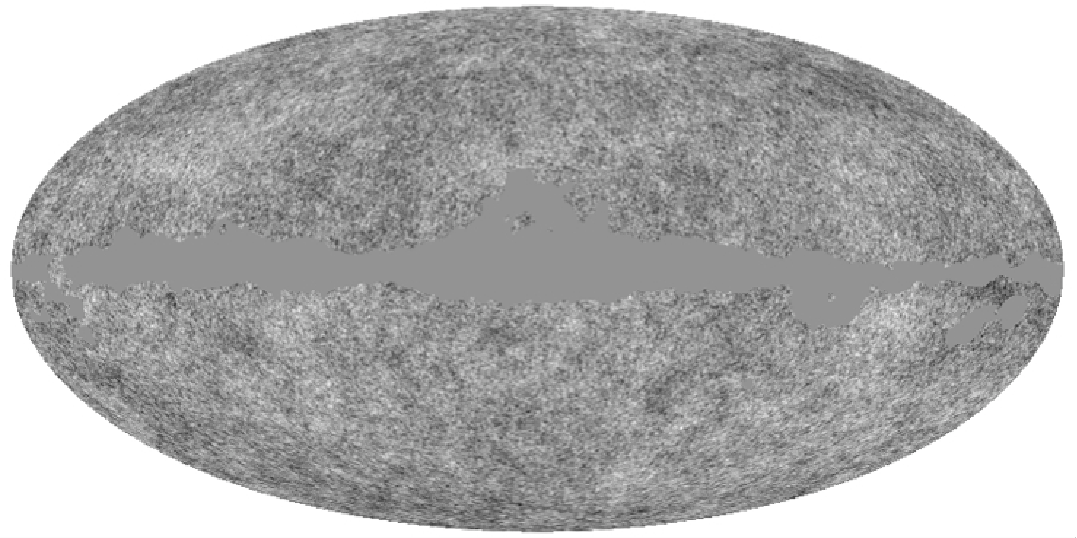
\includegraphics[width=7cm]{CMB_map}
% 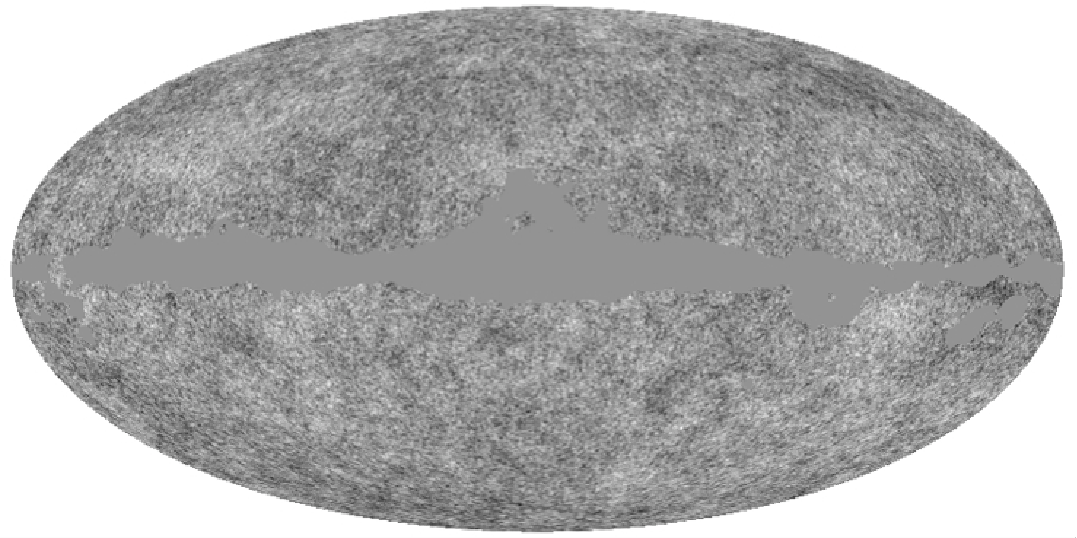
\includegraphics[width= 7cm]{CMB_w0db}
% 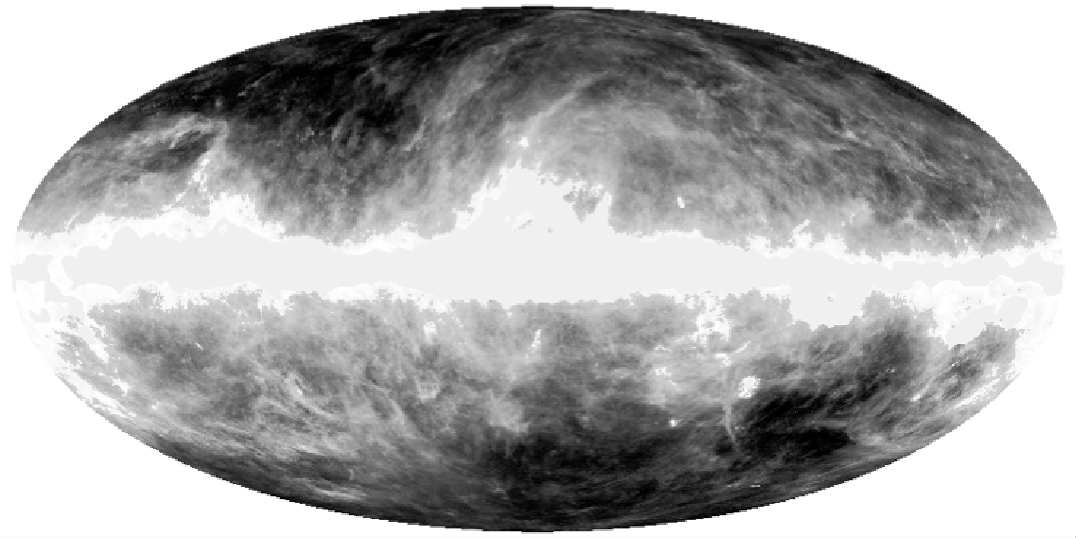
\includegraphics[width= 7cm]{hist_equal_dust}
% 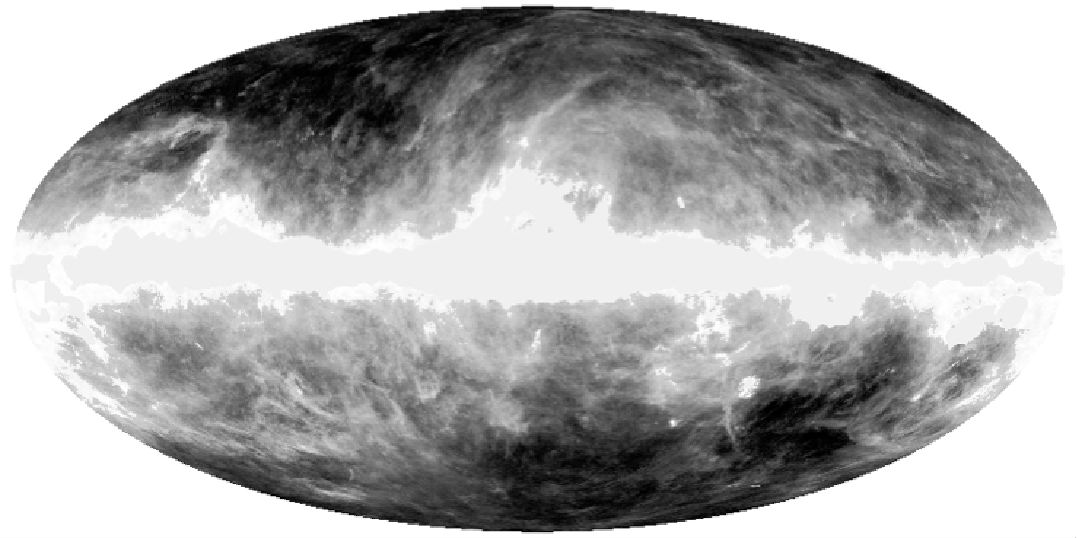
\includegraphics[width= 7cm]{hist_equal_dust_w_0db}
% 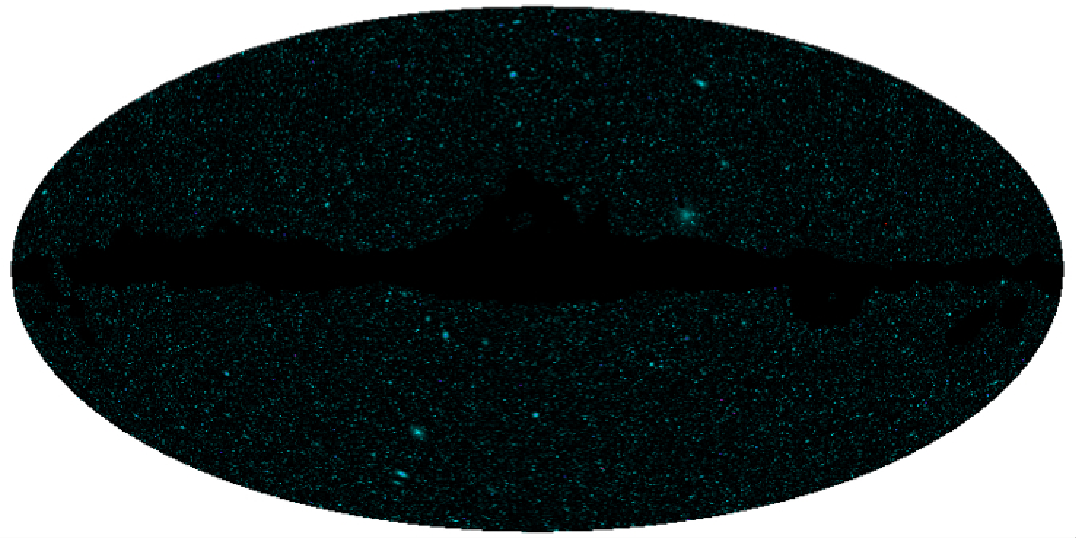
\includegraphics[width= 7cm]{sz_map3}
% 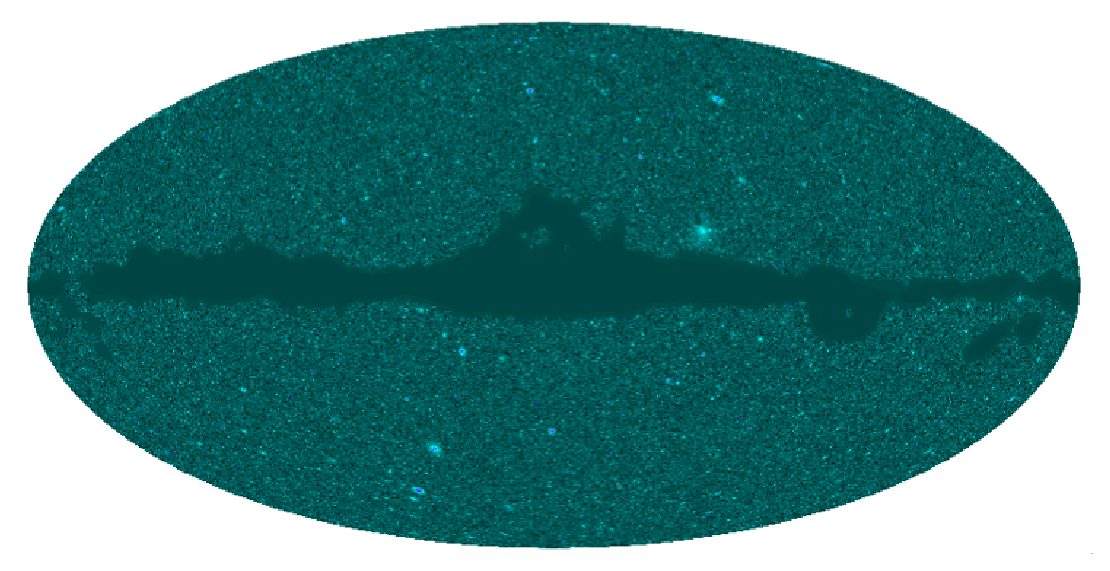
\includegraphics[width= 7cm]{sz_w_0db_bis}
% \caption{%%
% The maps on the left are the templates for CMB, galactic dust and SZ used in the experiment 
  % described in section~\ref{sec:NUMEXP}. The maps on the right were estimated using wSMICA 
  %  and scalewise Wiener filtering. (The different maps are drawn here in different color scales 
   % in order to enhance structures and ease visual comparisons).  } 
% \label{components}
% \end{center}
\vbox{
\centerline{
\hbox{
% \psfig{figure=CMB_w0db.ps,bbllx=0.5cm,bblly=7.5cm,bburx=21.5cm,bbury=20cm,width=7cm,clip=}
\psfig{figure=CMB_map.pdf,bbllx=0.5cm,bblly=7.5cm,bburx=21.5cm,bbury=20cm,width=7cm,clip=}
\psfig{figure=CMB_w0db.pdf,bbllx=0.5cm,bblly=7.5cm,bburx=21.5cm,bbury=20cm,width=7cm,clip=}
}}
\centerline{
\hbox{
\psfig{figure=hist_equal_dust.pdf,bbllx=0.5cm,bblly=7.5cm,bburx=21.5cm,bbury=20cm,width=7cm,clip=}
\psfig{figure=hist_equal_dust_w_0db.pdf,bbllx=0.5cm,bblly=7.5cm,bburx=21.5cm,bbury=20cm,width=7cm,clip=}
}}
\centerline{
\hbox{
\psfig{figure=sz_map3.pdf,bbllx=0.5cm,bblly=7.5cm,bburx=21.5cm,bbury=20cm,width=7cm,clip=}
\psfig{figure=sz_w_0db_bis.pdf,bbllx=0.5cm,bblly=7.5cm,bburx=21.5cm,bbury=20cm,width=7cm,clip=}
}}}
\caption{The maps on the left are zero mean templates for CMB ($\sigma =  4.17\times 10^{-5}$), galactic dust ($\sigma = 8.61\times 10^{-6}$) 
and SZ ($\sigma = 3.32\times 10^{-6}$) used in the experiment described in section~\ref{sect:NUMEXP}. The standard deviations given are for 
the region outside the galactic mask. The maps on the right were estimated using WSMICA and scalewise Wiener filtering as is explained in Appendix~2. 
Obviously, map reconstruction using Wiener filtering is optimal only in front of stationary Gaussian processes. For non Gaussian maps, such as 
given by the Sunyaev Zel'dovich effect, better reconstruction can be expected from non linear methods. The different maps are drawn here in 
different color scales in order to enhance structures and ease visual comparisons. }
\label{components}
\end{figure*}


\begin{figure}
\begin{center}
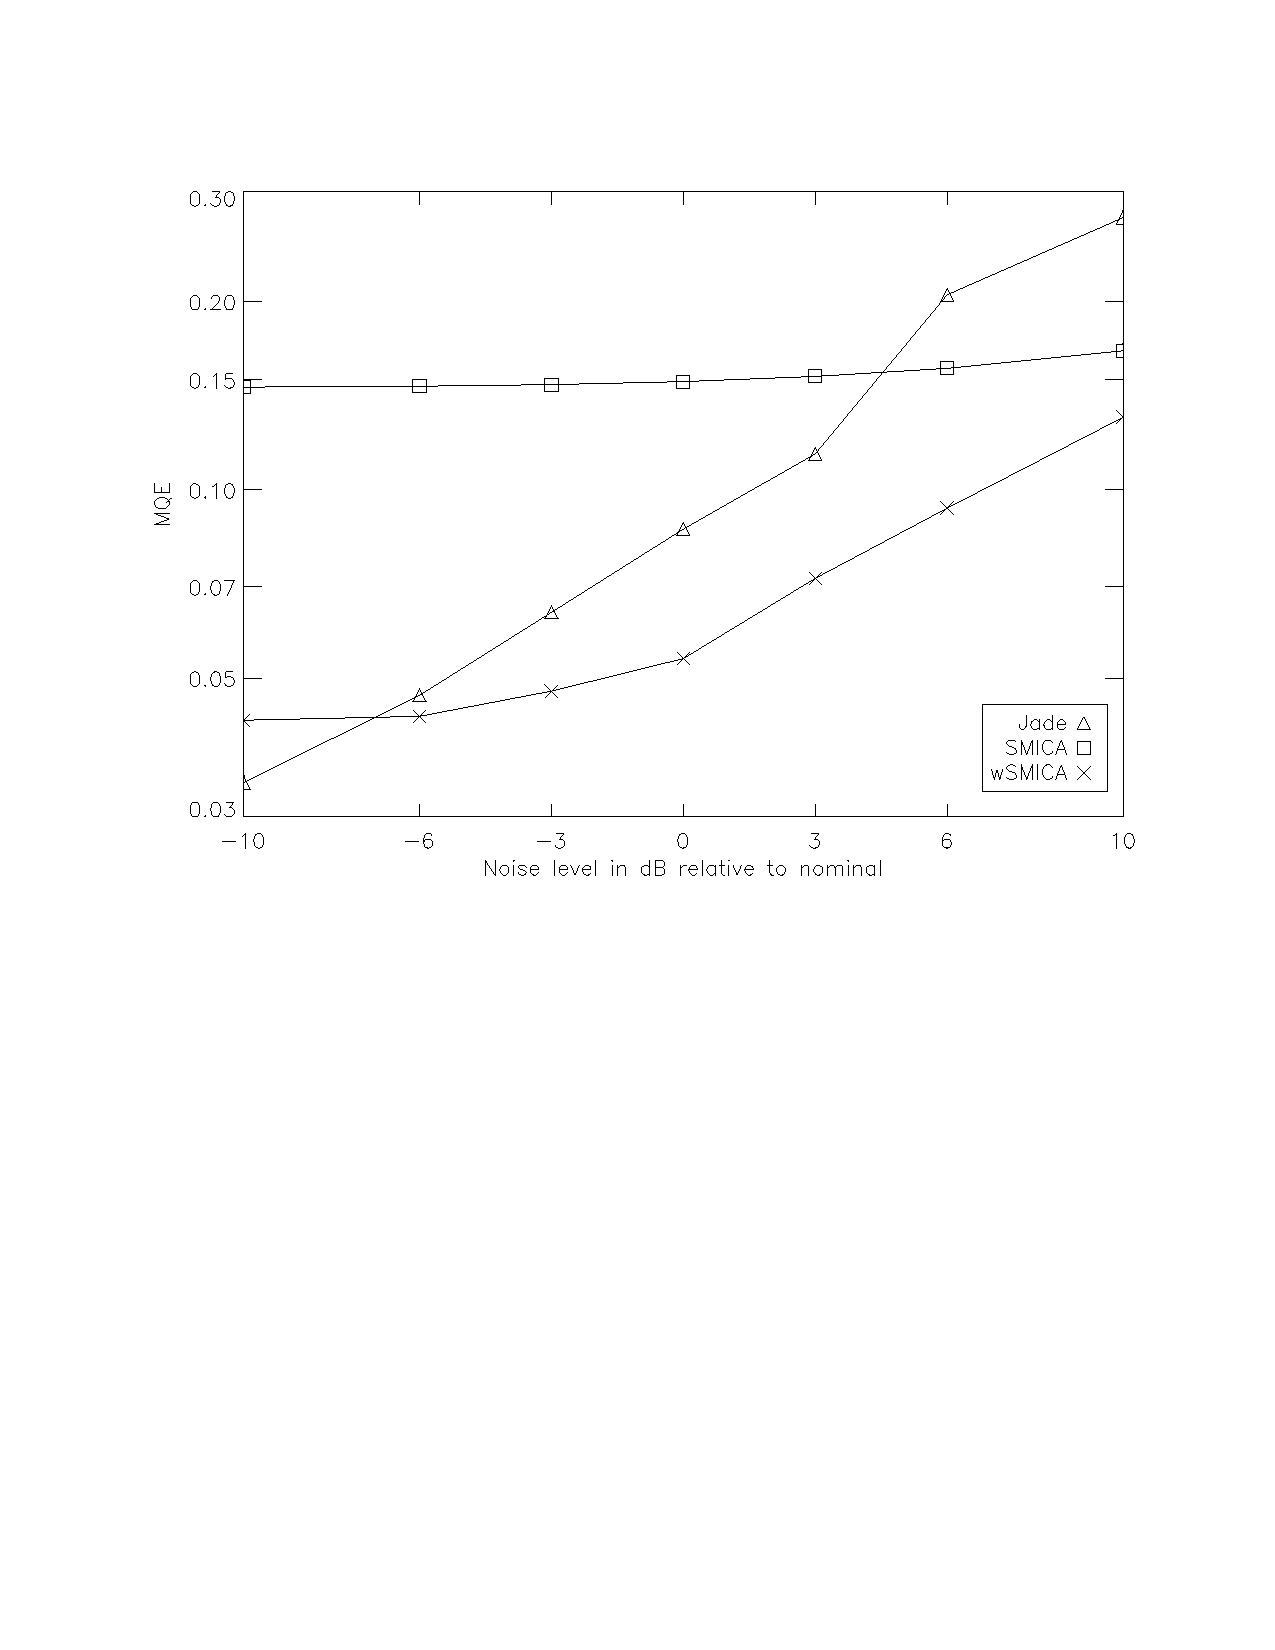
\includegraphics[width=8cm]{resultats_aa}
\caption{Relative reconstruction error defined by~(\ref{MQE}) of the CMB component map using SMICA, WSMICA and JADE as a function of the instrumental noise level in dB relative to the nominal values in table~\ref{NoiseScale}.} 
\label{resultats}
\end{center}
\end{figure}



\subsection{Sunyaev-Zeldovich cluster detection}

Another application of component separation techniques in astrophysics and cosmology is in the reconstruction of Sunyaev-Zel'dovich (SZ) 
galaxy clusters in future SZ-survey experiments such as Olimpo, APEX, or Planck which will use multiband bolometer cameras. The goal is 
to optimize SZ-Cluster extraction from the multichannel observed noisy maps. Resorting to blind methods is again attractive.

A complete description of the method we developed is given in~\cite{cluster:sz_cluster}. Before the actual detection of the SZ clusters, 
the multichannel data maps are combined and filtered to produce a clean map of the SZ component, with greater signal to noise ratio. We used 
an ICA approach to estimate the mixing matrix and perform the separation. A non linear filtering technique in the wavelet domain was used 
for the purpose of denoising. Finally a detection algorithm extracts the SZ clusters candidates from the restored SZ map. This is a new 
application of ICA to multichannel astrophysical data analysis. 

In the 100 to 600~GHz range, the brightest components of the sky are the Cosmic Microwave Background (CMB), the Infrared Point Sources, 
the Galactic dust emission and, swamped in the previous ones, the SZ clusters. It follows that the true sky map $X_{\nu}(\vartheta, \varphi)$, 
in a given optic band centered on $\nu$, can be modeled as a sum of distinct astrophysical radiations as in
\begin{equation} \label{SkyBandModel1}
	X_{\nu}(\vartheta, \varphi)  =  CMB_{\nu}(\vartheta, \varphi)  + IR_{\nu}(\vartheta, \varphi)  + Gal_{\nu}(\vartheta, \varphi)  + SZ_{\nu}(\vartheta, \varphi) 
\end{equation}
where $\vartheta, \varphi$ denote spatial or angular indexes on 2D or spherical maps. Assuming again that the radiative properties of the sources 
are completely isotropic in the sense that they do not depend on the direction of observation, the above model can be rewritten in the following factored form:
\begin{equation} \label{SkyBandModel2}
X_{\nu}(\vartheta, \varphi) =  \sum_{i} a_{\nu, i} S_{i}(\vartheta, \varphi)  \,\,+\,\, N_{\nu}(\vartheta, \varphi)
\end{equation}
where $S_{i}$ is the spatial template and $a_{\nu, i}$  the emission law of the $i\,{\textrm{th}}$ astrophysical component. Although this is 
a coarse approximation in the case of Infrared Point Sources, it is mostly valid for the other three components. With observations available 
in $m$ channels, assuming the beam varies only slightly as a function of $\nu$, equation~(\ref{SkyBandModel2}) can be written in matrix form : 
\begin{equation} \label{SkyBandModel3}
X(\vartheta, \varphi) = A\,\, S(\vartheta, \varphi)  \,\,+\,\, N(\vartheta, \varphi)
\end{equation}
where $X(\vartheta, \varphi)$ is a vector in $\mathbb{R}^m$, $A$ is an $m\times n$ matrix, n is the number of contributing astrophysical components, 
$S(\vartheta, \varphi)$ is now a vector in  $\mathbb{R}^n$ and $N(\vartheta, \varphi)$ in $\mathbb{R}^m$. Equation~(\ref{SkyBandModel3}) expresses 
that the observations consist of linear mixtures of astrophysical components with different weights and additive noise. 

Simulations of the major contributions in the frequency range considered here were generated according to the procedure described 
in~\cite{cluster:sz_cluster}. Figure~\ref{RawMaps} shows such typical simulations. These four physical components are linearly 
combined into a ``true" sky maps which are then convolved  with the experimental beam. Then instrumental noise is added. The resulting 
noisy mixture maps, as shown on figure~\ref{NoisyMaps} would be what the analysis team would recover from the data, after pointing 
reconstruction, outlier removal, de-correlation of instrumental systematics in the data, and map-making. 

\begin{figure*}[htp]
\vbox{
\centerline{
\hbox{
\psfig{figure=CMB.pdf,bbllx=3.cm,bblly=6.cm,bburx=19.1cm,bbury=21.7cm,height=7.5cm,width=6.5cm,clip=}
\hspace{0.2cm}
\psfig{figure=SZOld.pdf,bbllx=3.cm,bblly=6.cm,bburx=19.1cm,bbury=21.7cm,height=7.5cm,width=6.5cm,clip=}
}}
\vspace{0.3cm}
\centerline{
\hbox{
\psfig{figure=IR.pdf,bbllx=3.cm,bblly=6.cm,bburx=19.1cm,bbury=21.7cm,height=7.5cm,width=6.5cm,clip=}
\hspace{0.2cm}
\psfig{figure=TheGalax.pdf,bbllx=3.cm,bblly=6.cm,bburx=19.1cm,bbury=21.7cm,height=7.5cm,width=6.5cm,clip=}
}}
}
\caption{The 4 physical components of the sky included in our simulation: 
{\bf a)} is a map of the CMB's anisotropies in unit of $\mu$K, 
{\bf b)} is the SZ Cluster map, in unit of y Compton, 
{\bf c)} is the IR point source map, convolved with a beam of 2 arcmin, in Jy at 350GHz, finally 
{\bf d)} is the Galactic dust map in unit of MJy/st at 100 $\mu$m.}
\label{RawMaps}
\end{figure*}



%
%
%
\begin{figure*}[htp]
\vbox{
\centerline{
\hbox{
\psfig{figure=c143GHz.pdf,bbllx=3.cm,bblly=6.cm,bburx=19.1cm,bbury=21.7cm,height=7.0cm,width=6.0cm,clip=}
\hspace{0.2cm}
\psfig{figure=c217GHz.pdf,bbllx=3.cm,bblly=6.cm,bburx=19.1cm,bbury=21.7cm,height=7.0cm,width=6.0cm,clip=}
}}
\vspace{0.2cm}
\centerline{
\hbox{
\psfig{figure=c385GHz.pdf,bbllx=3.cm,bblly=6.cm,bburx=19.1cm,bbury=21.7cm,height=7.0cm,width=6.0cm,clip=}
\hspace{0.2cm}
\psfig{figure=c600GHz.pdf,bbllx=3.cm,bblly=6.cm,bburx=19.1cm,bbury=21.7cm,height=7.0cm,width=6.0cm,clip=}
}}
}
\caption{Simulated maps in Olimpo's four frequency bands. {\bf upper right} is the 147 GHz Band, {\bf upper left)} is the 217 GHz Band, {\bf lower right} is 
the 385 GHz Band: CMB anisotropies, IR point sources and Galactic Dust blend in this band {\bf lower left} 500 GHz: IR point sources and Galactic Dust are 
the dominant features at high frequencies. SZ cluster signal is dominated by other astrophysical sources at all frequencies.}
\label{NoisyMaps}
\end{figure*}
%
%
%



Any mainstream ICA algorithm for sparse sources, based on maximizing non-Gaussianity, would probably be successful at separating the SZ component map. 
We chose to use JADE in the wavelet domain, as described in section~\ref{sec:wjade}. Wavelets come into play as a sparsifying transform : data is sparse 
on a basis when this basis allows to describe that signal with a small number of coefficients. This is a highly desirable property, since noise is not 
expected to be sparse at the same time on such a basis. Choosing a sparsifying basis thus allows to enhance signal to noise ratio. Moving the data to 
a wavelet representation does not affect its information content and applying a wavelet transform on both sides of~(\ref{model0}) does not affect the 
mixing matrix and the model structure is preserved. However, the statistical distribution of the data coefficients in the new representation is different: 
wavelets are known to lead to sparse approximately \emph{i.i.d.} representations of structured data. Further, the \emph{local} (coefficient wise) signal 
to noise ratio depends on the choice of a representation. A wavelet transform tends to grab the informative coherence between pixels while averaging 
the noise contributions, thus enhancing structures in the data. Although the standard ICA model is for a noiseless setting, the derived methods can be 
applied to real data. Performance will depend on the detectability of significant coefficients \emph{i.e.} on the sparsity of the statistical distribution 
of the coefficients. Moving to a wavelet representation will then often lead to more robustness to noise. We noted that the estimation of the mixing matrix 
could be slightly enhanced by prefiltering the data using a Gaussian with the same width as the optical beam. The resulting SZ component map is shown 
on figure~\ref{JADEMaps}. Different filtering techniques were applied on this map and the results of a quantitative comparison are given in~\cite{cluster:sz_cluster}.




\begin{figure}[htp]
 \centerline{
\hbox{
%\psfig{figure=SZJadeG1_69w.ps}
\psfig{figure=SZJadeG1_69w.pdf,bbllx=3.cm,bblly=6.cm,bburx=19.1cm,bbury=21.8cm,height=6.5cm,width=6.5cm,clip=}
}
}
\caption{SZ component map extracted by JADE from the four observed noisy maps. The SZ cluster signal, subdominant at all observed frequencies, 
now appears clearly. No obvious leftovers from other astrophysical sources are seen. \textbf{Remaining noise is small, because we prefiltered 
data before JADE processing, and we simulated the nominal noise levels of an ambitious project: Olimpo.}}
\label{JADEMaps}
\end{figure}


 
